\chapter{Measurements}\label{ch:measurements}

\section{Recordings}

As mentioned above, we used a sample recording of a wooden stick hitting every different area on the objects, to extract the necessary data. We separated the objects into areas depending on their shape and tried to keep the struck sound as uniform as possible inside the same area. 

As the hitting object we used a drumstick shown in the figure \ref{fig:drumstick}. All recordings took place in the same room, using the same drumstick and the same hitting force. The only parameter changing every time are the point of the object being struck.

\begin{figure}[H]
  \centering
    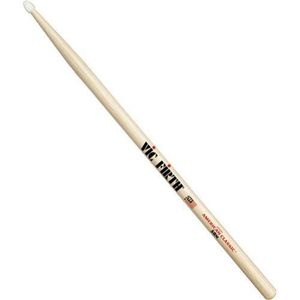
\includegraphics[width=0.3\textwidth]{drumstick.jpg}
      \caption{The drumstick used to struck objects during recordings.}
      \label{fig:drumstick}
\end{figure}

We used eleven different objects of everyday life. The idea of choosing those objects came firstly from the need of both owning the object (to perform the recording) and also being able to model it for the demo (simple enough objects). Secondly, since we wanted to test the immersion of the synthesized sounds on users, we wanted to be sure that the sounds used are familiar to them. In figure \ref{fig:objects} both real and modeled objects are pictured. 

\begin{figure}[H]
    \centering
    \begin{subfigure}[b]{0.7\textwidth}
        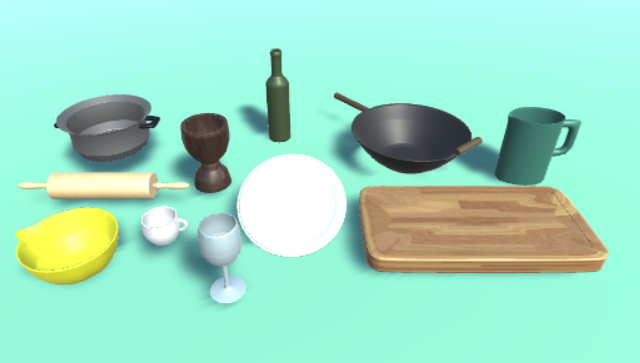
\includegraphics[width=\textwidth]{realobjects.PNG}
        \caption{Real objects.}
        \label{fig:gull}
    \end{subfigure}
    ~ %add desired spacing between images, e. g. ~, \quad, \qquad, \hfill etc. 
      %(or a blank line to force the subfigure onto a new line)
    \begin{subfigure}[b]{0.7\textwidth}
        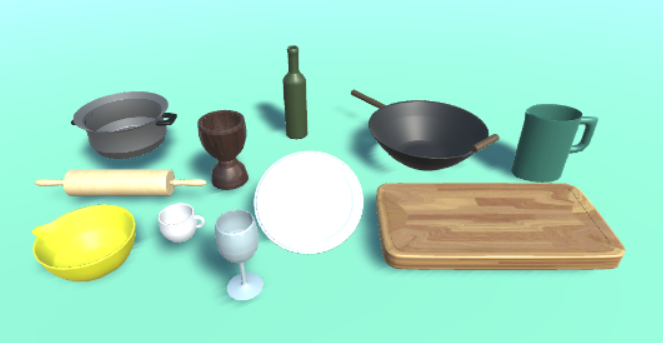
\includegraphics[width=\textwidth]{3dobjects.PNG}
        \caption{3D models of the objects.}
        \label{fig:tiger}
    \end{subfigure}
    \caption{The eleven objects used in the thesis.}\label{fig:objects}
\end{figure}

For the recordings we used a \Todo{describe the device used for recordings}. For the 3D models we used Maya Autodesk software \cite{bib:maya} and exported them as FBX\textregistered\ files \cite{bib:fbx}, a file format recognizable by Unity\textregistered\ software \cite{bib:unity}.

\section{User tests}

To examine the immersion of real-time produced and physics-based sounds on game players, we performed some tests to people. The stimuli of the test was both a recorded sound of a struck object and its corresponding synthesized sound using both sinusoidal and filter-based synthesis.